\chapter{Método} \label{chap:metodo}

% Objetivo: documentar o método de forma reproduzível: dados, features, alvo,
% protocolo temporal, TFT, baselines, métricas, explicabilidade e regra de decisão.

\section{Desenho da pesquisa}
Esta pesquisa adota abordagem quantitativa, aplicada e de natureza experimental-computacional, com foco em previsão probabilística de retornos diários sob controle de validade metodológica. O desenho é confirmatório: um único candidato --- o TFT treinado com todas as \textit{features} do registro, com hiperparâmetros congelados após uma busca exploratória --- é comparado a uma hierarquia pré-declarada de \textit{baselines}, sem qualquer seleção por desempenho fora da amostra. As decisões de desenho foram formuladas como escolhas metodológicas para reduzir vieses de avaliação e preservar a reprodutibilidade dos resultados \cite{PINEAU2021REPRODUCIBILITY}.

O fluxo geral é sequencial: ingestão dos dados brutos, engenharia de \textit{features}, construção do conjunto de dados, treinamento do candidato e dos \textit{baselines} sob o mesmo protocolo temporal, persistência das previsões fora da amostra e, por fim, cálculo das métricas, testes estatísticos e regra de decisão pré-registrada. Os experimentos dividem-se em duas rodadas de natureza distinta \cite{RASCHKA2018}: uma \textbf{rodada exploratória} de busca de hiperparâmetros, que não constitui evidência, e uma \textbf{rodada confirmatória}, executada uma única vez com a configuração congelada.

\section{Dados}
Os dados combinam quatro fontes, todas com granularidade diária e \textit{timestamps} padronizados em UTC: (i) cotações OHLCV diárias de AAPL, obtidas via \texttt{yfinance}; (ii) notícias sobre o ativo, obtidas da API Alpha Vantage; (iii) demonstrativos contábeis trimestrais (resultado, balanço e fluxo de caixa) e datas de divulgação de resultados, também da Alpha Vantage; e (iv) o calendário de pregão da bolsa de Nova York (XNYS), que define as sessões válidas, os feriados e o horário de fechamento. O calendário é a referência temporal de todo o trabalho: horizontes, purga e embargo são contados em sessões de pregão, e não em dias corridos.

O sentimento das notícias é estimado pelo modelo FinBERT \cite{ARACI2019}, com os pesos fixados em uma revisão específica do repositório de modelos para garantir reprodutibilidade. O escore de cada notícia é \(P(\text{positivo}) - P(\text{negativo})\), e os escores são agregados por sessão de pregão.

Os dados brutos são preservados de forma imutável; todas as \textit{features}, previsões e métricas são derivadas deles de forma determinística. O ativo e a janela temporal são parâmetros da execução, registrados na assinatura de configuração de cada \textit{run}.

\section{Engenharia de \textit{features}}
As \textit{features} são organizadas em quatro famílias fixas, exigidas pela hipótese H3: preço, técnico, sentimento e fundamento. O registro contém 55 \textit{features} (Tabela~\ref{tab:familias}), cada uma declarada com sua família, colunas de origem, fórmula, período de aquecimento (\textit{warmup}), tipagem para o TFT e uma \textit{tag} obrigatória de causalidade; uma \textit{feature} sem contrato de causalidade é rejeitada pelo registro. O conjunto de \textit{features} utilizado é identificado por um \textit{hash} do conteúdo do registro, que integra a identidade de cada execução.

\begin{table}[htb]
\centering
\caption{Famílias de \textit{features} do registro}
\label{tab:familias}
\small
\begin{tabular}{p{2.3cm} p{1.2cm} p{10cm}}
\toprule
Família & Qtd. & Exemplos \\
\midrule
Preço & 17 & OHLCV; log-retornos de 1, 5 e 21 dias; \textit{momentum} de 5, 21 e 63 dias; reversão; \textit{drawdown}; proxy de iliquidez de Amihud; \textit{z-score} e sinal de pico de volume \\
Técnico & 17 & RSI(14) de Wilder; MACD e linha de sinal; médias exponenciais de 10, 50, 100 e 200 sessões; volatilidade de 20 dias, Parkinson e Garman-Klass; semivolatilidade negativa; volatilidade da volatilidade; regimes de volatilidade e de tendência \\
Sentimento & 11 & escore médio, desvio-padrão e volume de notícias; defasagens de 1, 3 e 5 sessões; média exponencial; surpresa de sentimento; interações com volatilidade e volume \\
Fundamento & 10 & receita, lucro líquido, fluxo de caixa operacional, patrimônio líquido e passivo total; margem líquida, alavancagem, eficiência de caixa; crescimento anual de receita e de lucro \\
\bottomrule
\end{tabular}
\fonte{Elaborado pelo autor (2026).}
\end{table}

A causalidade é garantida por regras verificadas por teste, e não por convenção:
\begin{itemize}
    \item \textbf{Indicadores e derivadas} usam janelas estritamente retrospectivas que terminam na própria sessão; cada indicador é conferido contra sua fórmula canônica e contra um teste de invariância: acrescentar sessões futuras à série não altera nenhum valor passado.
    \item \textbf{Sentimento} respeita o corte de fechamento: uma notícia publicada após o fechamento da sessão é atribuída à próxima sessão de pregão, nunca a uma sessão já encerrada.
    \item \textbf{Fundamentos} entram por junção \textit{as-of} retrospectiva pela data efetiva de disponibilidade, que é a data de divulgação do resultado ou, na sua ausência, o fim do período fiscal acrescido de 45 dias corridos; uma data efetiva posterior à sessão da amostra interrompe a execução com erro.
    \item \textbf{Tipagem para o TFT}: todas as \textit{features} do registro são \textit{observadas} (desconhecidas no futuro); apenas o dia da semana e o mês são \textit{conhecidos}.
\end{itemize}

Cada \textit{feature} declara seu período de aquecimento, e um \textit{gate} de qualidade verifica, sobre o conjunto final, que o primeiro valor válido de cada \textit{feature} não ocorre depois do aquecimento declarado e que a fração de valores ausentes após o aquecimento é aceitável.

O candidato confirmatório é \textit{all-features}: todas as \textit{features} habilitadas no registro, sem seleção por desempenho fora da amostra. Essa escolha elimina a busca em vez de corrigi-la \cite{WHITE2000,ROMANOWOLF2005}: as correções de múltiplas comparações passam a operar sobre uma família pequena e congelada de hipóteses. A contribuição relativa das famílias é objeto descritivo de H3, e não critério de seleção.

\section{Alvo e alinhamento temporal}
O alvo é o retorno logarítmico de um dia, \(r_t = \log(P_t / P_{t-1})\), em que \(P_t\) é o preço de fechamento da sessão \(t\). A linha do conjunto de dados indexada em \(t\) é a sessão de decisão: carrega as \textit{features} conhecidas até \(t\). Para o horizonte \(h\), o valor previsto na decisão \(t\) é o retorno de \textbf{um} dia realizado na sessão \(t+h\), e o \textit{target timestamp} é a sessão localizada \(h\) posições à frente na grade de sessões de pregão --- nunca \(h\) dias corridos, o que faria, por exemplo, uma decisão de sexta-feira apontar para um sábado. Como o alvo em \(h\) é um retorno diário, e não o retorno acumulado de \(h\) dias, nenhuma regra de escala \(\sqrt{h}\) se aplica aos comparadores.

\section{Protocolo experimental}
A validação é \textit{walk-forward} de janela expansiva \cite{TASHMAN2000,HYNDMANATHANASOPOULOS2021}: o treino de cada \textit{fold} começa na primeira sessão disponível e cresce a cada \textit{fold}, enquanto os blocos de teste ladrilham a cauda da série em blocos contíguos e disjuntos. A janela expansiva foi preferida à deslizante porque aproveita todo o histórico de uma série única e relativamente curta; a não estacionariedade é tratada pelo re-ajuste por \textit{fold}, pelo embargo e pela recência do conjunto de calibração.

Cada \textit{fold} tem quatro partições disjuntas e temporalmente ordenadas (Figura~\ref{fig:walkforward}): \texttt{train} (ajuste), \texttt{early\_stop} (monitoramento da parada antecipada), \texttt{calib} (calibração conformal) e \texttt{test} (avaliação fora da amostra). Entre partições consecutivas há um intervalo de \(h_{\max}\) + embargo sessões excluídas: a purga de \(h_{\max}\) sessões impede que o alvo de uma decisão, realizado até \(h_{\max}\) sessões depois, caia no bloco seguinte, e o embargo corta a dependência serial na fronteira \cite{LOPEZDEPRADO2018}. O bloco \texttt{calib} é o mais recente antes do teste e \textbf{nunca} é usado para ajuste, parada antecipada ou seleção de modelo, pois a validade da calibração conformal depende de um conjunto disjunto de tudo o que ajustou ou selecionou o modelo \cite{ROMANO2019CQR}. As quatro partições de cada \textit{fold} compõem sua impressão digital.

\begin{figure}[htb]
\centering
\caption{Geometria de um \textit{fold} do \textit{walk-forward}}
\label{fig:walkforward}
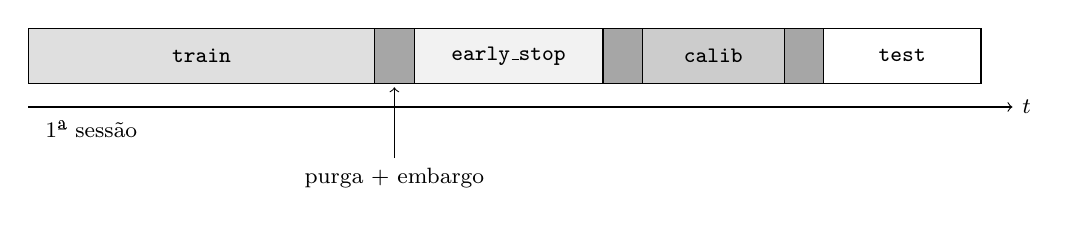
\begin{tikzpicture}[x=1cm,y=1cm,font=\footnotesize]
  \draw[fill=gray!25] (0,0) rectangle (4.4,0.7) node[midway] {\texttt{train}};
  \draw[fill=gray!70] (4.4,0) rectangle (4.9,0.7);
  \draw[fill=gray!10] (4.9,0) rectangle (7.3,0.7) node[midway] {\texttt{early\_stop}};
  \draw[fill=gray!70] (7.3,0) rectangle (7.8,0.7);
  \draw[fill=gray!40] (7.8,0) rectangle (9.6,0.7) node[midway] {\texttt{calib}};
  \draw[fill=gray!70] (9.6,0) rectangle (10.1,0.7);
  \draw[fill=white] (10.1,0) rectangle (12.1,0.7) node[midway] {\texttt{test}};
  \draw[->] (0,-0.3) -- (12.5,-0.3) node[right] {\(t\)};
  \node[below] at (0.8,-0.35) {1ª sessão};
  \draw[->] (4.65,-0.95) -- (4.65,-0.05);
  \node[below] at (4.65,-0.95) {purga + embargo};
\end{tikzpicture}
\fonte{Elaborado pelo autor (2026).}
\end{figure}

A variância entre execuções é tratada como parte do resultado \cite{BOUTHILLIER2021}: a rodada confirmatória repete o treino sob múltiplas sementes em cada \textit{fold}, e a avaliação com múltiplas origens temporais é mais robusta que o \textit{holdout} único de fim de série \cite{TASHMAN2000,BERGMEIR2012}. Quando \textit{folds} sucessivos produzem mais de uma previsão para o mesmo ponto alinhado, mantém-se apenas a operacionalmente mais recente, garantindo uma observação por ponto; um empate exato interrompe a execução em vez de ser resolvido arbitrariamente. O candidato, os comparadores, as sementes, os \textit{folds} e a configuração compõem o cohort confirmatório, que é congelado e \textit{hasheado} antes da execução e identificado por um id de coorte comum a todas as suas execuções.

\section{Configuração do modelo TFT}
O TFT opera exclusivamente em modo quantílico: a função de perda é a soma da \textit{pinball loss} sobre os níveis da grade e sobre os passos do decodificador \cite{LIMETAL2021TFT}. Em cada \textit{fold}, um único modelo é ajustado com decodificador de \(h_{\max}\) passos, e os horizontes de interesse são lidos dos passos correspondentes. A janela de contexto do codificador termina na própria sessão de decisão e pode alcançar sessões de partições anteriores; o que nunca atravessa a fronteira das partições é o ajuste e a seleção. Coerentemente, o normalizador do alvo é um padronizador global ajustado apenas no bloco de treino e herdado pelas demais partições.

A parada antecipada monitora a perda no bloco \texttt{early\_stop}, e a previsão usa os pesos da época de menor perda de validação, e não os da última época \cite{PRECHELT1998}. Os hiperparâmetros (tamanho da janela de contexto, dimensão oculta, número de cabeças de atenção, \textit{dropout}, taxa de aprendizado, tamanho de lote) são explorados na rodada exploratória com Optuna e amostrador TPE \cite{AKIBA2019}, avaliando cada tentativa apenas pela perda no bloco \texttt{early\_stop}; nenhuma previsão fora da amostra é persistida nessa rodada. A configuração escolhida é então congelada para a rodada confirmatória \cite{RASCHKA2018}.

\section{\textit{Baselines}}
A comparação contra \textit{baselines} explícitos é componente metodológico central. Adota-se uma hierarquia em três níveis, que sobe em informação distribucional:
\begin{itemize}
    \item \textbf{Naive.} \textit{Retorno nulo}, equivalente ao passeio aleatório sem \textit{drift} do log-preço \cite{CAMPBELL1997}: sob esse modelo o retorno de um dia previsto é zero para todo horizonte; e \textit{média histórica}, a média dos retornos do bloco de treino. Ambos emitem uma grade degenerada, em que todos os níveis recebem o mesmo valor.
    \item \textbf{Estatísticos.} \textit{AR(1)}, com quantis gaussianos obtidos da média e da variância de previsão a \(h\) passos em forma fechada \cite{HAMILTON1994}; \textit{EWMA-vol}, volatilidade condicional da RiskMetrics com \(\lambda = 0{,}94\) e média nula, com quantis gaussianos \cite{RISKMETRICS1996,MCNEIL2005}; e \textit{quantis empíricos históricos}, quantis amostrais do tipo 7 de \cite{HYNDMANFAN1996} sobre uma janela deslizante de 252 sessões.
    \item \textbf{Modelo de aprendizado de máquina.} \textit{Gradient boosting} quantílico \cite{FRIEDMAN2001} com LightGBM \cite{KE2017LIGHTGBM}: um modelo independente por par (nível de quantil, horizonte), treinado com a \textit{pinball loss} sobre o rótulo \(r_{t+h}\), com as mesmas \textit{features} do candidato mais o calendário como inteiros ordinais, e parada antecipada pelo número de iterações que minimiza a \textit{pinball} média da grade no bloco \texttt{early\_stop}.
\end{itemize}

Os parâmetros dos \textit{baselines} estatísticos são estimados uma única vez por \textit{fold}, no bloco de treino, e apenas o estado condicionante (o último retorno do AR(1), a recursão da variância EWMA, o conteúdo da janela deslizante) avança causalmente até cada decisão --- o mesmo protocolo de informação do candidato. Todos os comparadores emitem a mesma grade de níveis do candidato, sob as mesmas partições, e suas previsões são persistidas no mesmo formato e na mesma coorte, permitindo análise pareada por \textit{target timestamp}. Os cinco \textit{baselines} estatísticos são monotônicos por construção; o GBM, por treinar um modelo por nível, pode cruzar e recebe o mesmo rearranjo aplicado ao candidato. A grade degenerada dos \textit{baselines} naive é penalizada nos níveis extremos pela \textit{pinball}, o que é informativo: um previsor pontual equivale, em regras de pontuação, a uma distribuição concentrada em um ponto \cite{GNEITING2007}.

\section{Métricas de avaliação} \label{sec:metricas}
A avaliação probabilística considera a \textit{pinball loss} média sobre a grade (Equação~\ref{eq:pinball}) como métrica primária e o CRPS (Equação~\ref{eq:crps}) como complementar; a calibração marginal por quantil (Equação~\ref{eq:coverage}) e o \textit{reliability diagram}; o PICP (Equação~\ref{eq:picp}) e o MPIW (Equação~\ref{eq:mpiw}) de intervalos definidos por pares de níveis da grade; o \textit{interval score} de Winkler; e a cobertura condicional pelos testes de Christoffersen e Kupiec. Todas as métricas são apuradas separadamente por horizonte e nunca agregadas entre horizontes. As métricas pontuais (RMSE, MAE, acurácia direcional) são registradas apenas como perfil descritivo, sem papel no veredito, pelas razões expostas no Capítulo~\ref{chap:intro}.

Para cada previsão e cada nível persistem-se o valor bruto do modelo, o valor após o rearranjo monotônico e um indicador de que o rearranjo alterou a ordem. A variante que alimenta cada métrica confirmatória é fixada no pré-registro; a outra permanece disponível para quantificar o efeito do rearranjo. Separadamente, um \textit{gate} de degeneração identifica previsões cuja grade colapsou (\(\hat{q}_{\tau_1} = \hat{q}_{\tau_K}\)), que não carregam informação distribucional: as métricas dessas linhas são invalidadas e a taxa de degeneração é reportada por execução. O rearranjo corrige ordem sem mascarar colapso; o \textit{gate} detecta colapso sem alterar ordem.

A comparação entre modelos usa o teste de Diebold-Mariano (Equação~\ref{eq:dm}) unilateral sobre a \textit{pinball loss}, com variância HAC de defasagem \(h-1\) e correção HLN, ajuste de Holm sobre a família de comparações e \textit{Model Confidence Set} com \textit{bootstrap} em blocos. A calibração nativa do TFT é confrontada com intervalos obtidos por CQR calibrada no bloco \texttt{calib} de cada \textit{fold} e horizonte, com cobertura reportada como empírica. O VaR é reportado de forma descritiva, sobre a variante rearranjada, com \textit{backtest} de exceções.

Cada métrica e cada teste estatístico são validados contra implementações de referência --- R (\texttt{forecast::dm.test}, \texttt{rugarch::VaRTest}), \texttt{scikit-learn}, \texttt{scoringrules}, \texttt{arch} e \texttt{statsmodels} --- e contra casos analíticos com resultado conhecido, de modo que nenhum número reportado depende de uma implementação não conferida.

\section{Explicabilidade e contribuição de famílias}
A contribuição relativa das famílias de \textit{features} (H3) é caracterizada por três métodos: os pesos da \textit{Variable Selection Network} nativa do TFT \cite{LIMETAL2021TFT}; a importância por permutação \cite{BREIMAN2001} por família, medida como aumento da \textit{pinball loss} quando a família é permutada, com intervalo de confiança por \textit{bootstrap}; e a ablação, em que o modelo é re-treinado sem cada família. Uma afirmação de contribuição relativa exige consistência em pelo menos dois dos três métodos, por horizonte; divergências entre métodos são reportadas como instabilidade da contribuição, e não como falha do estimador.

A análise é preditiva e condicional ao modelo treinado, não causal: os três métodos indicam o que o modelo usou, não o que move o retorno. Conclusões são extraídas de evidência global por horizonte e da estabilidade entre sementes e \textit{folds}; interpretações por instância são apenas ilustrativas.

\section{Rastreabilidade e governança de coorte}
Cada execução é identificada pelo \textit{hash} determinístico descrito no Capítulo~\ref{chap:fundamentacao}, e registra a assinatura de configuração, a impressão digital das partições, a semente, o \textit{fold}, a versão do modelo e o id da coorte. A coorte é definida pelo ativo, pelo conjunto de \textit{features}, pelo horizonte máximo --- que fixa a largura da purga --- e pelo id de coorte; comparações e agregações são sempre feitas dentro de uma coorte, e comparações fora dela não são reportadas. Falhas de execução são registradas com etapa e tipo de erro, e não silenciosamente descartadas.

Como todas as tabelas analíticas são derivadas das previsões persistidas, qualquer reanálise --- inclusive com outra variante quantílica ou outro parâmetro de teste --- é reconstruída sem re-treinar os modelos. Os detalhes de implementação estão no Apêndice D.

\section{Critérios de qualidade}
Os critérios de qualidade incluem integridade temporal (grade de sessões estritamente crescente, sem sobreposição entre partições), unicidade das chaves de previsão por execução, horizonte, \textit{target timestamp} e nível, monotonicidade da variante rearranjada ao longo dos \(K\) níveis e a taxa de degeneração da grade, cujo limiar de aceitação é fixado no pré-registro. Somente são aceitas comparações pareadas com interseção temporal exata entre modelos.

\subsection{\textit{Scorecard} pré-registrado} \label{sec:scorecard}
A barreira entre execução experimental e afirmação científica é um \textit{scorecard} pré-registrado aplicado mecanicamente, em quatro etapas:
\begin{enumerate}
    \item \textbf{Validade estatística}: a perda pareada é a \textit{pinball loss}; não há seleção dos melhores \textit{runs}; a família de Holm é restrita a comparações sobre as mesmas partições; a série de perdas está deduplicada e alinhada.
    \item \textbf{Calibração (H1)}: coberturas por nível e PICP dentro das bandas pré-registradas, por horizonte; um horizonte reprovado aqui não entra na comparação de \textit{skill}.
    \item \textbf{\textit{Skill} relativo (H2)}: DM com ajuste de Holm por horizonte contra cada nível da hierarquia de \textit{baselines}, e pertencimento ao MCS.
    \item \textbf{Contribuição (H3)}: consistência em pelo menos dois de três métodos.
\end{enumerate}
O veredito só é emitido com todas as condições de validade satisfeitas. As demais métricas compõem um perfil comparativo que nunca altera o veredito, e nada é agregado entre horizontes.

Os limiares numéricos do \textit{scorecard} pertencem a três categorias, e essa distinção é explicitada para que sua magnitude não seja confundida com valor canonizado pela literatura: convenções estatísticas consagradas (como o nível de significância \(\alpha = 0{,}05\)); bandas de calibração e limiares de qualidade sem valor canônico na literatura, cuja validade decorre da declaração antecipada; e parâmetros dos procedimentos (por exemplo, o tamanho de bloco do \textit{bootstrap} do MCS). Todos são fixados no pré-registro antes da rodada confirmatória, e qualquer alteração posterior invalida o \textit{hash} do pré-registro.
